\paragraph{Introduction}
    USGS provides an almost real-time environment to gather multiple parameters from water in/nearby the United States, i.e., water temperature, pH, salinity, and specific conduction.
    
    It provides the data in tab-separated \textit{.rdb} files with more information about the format available at \href{https://help.waterdata.usgs.gov/faq/about-tab-delimited-output}{waterdata.usgs.gov}.

    \begin{figure}[H]
        \centering
        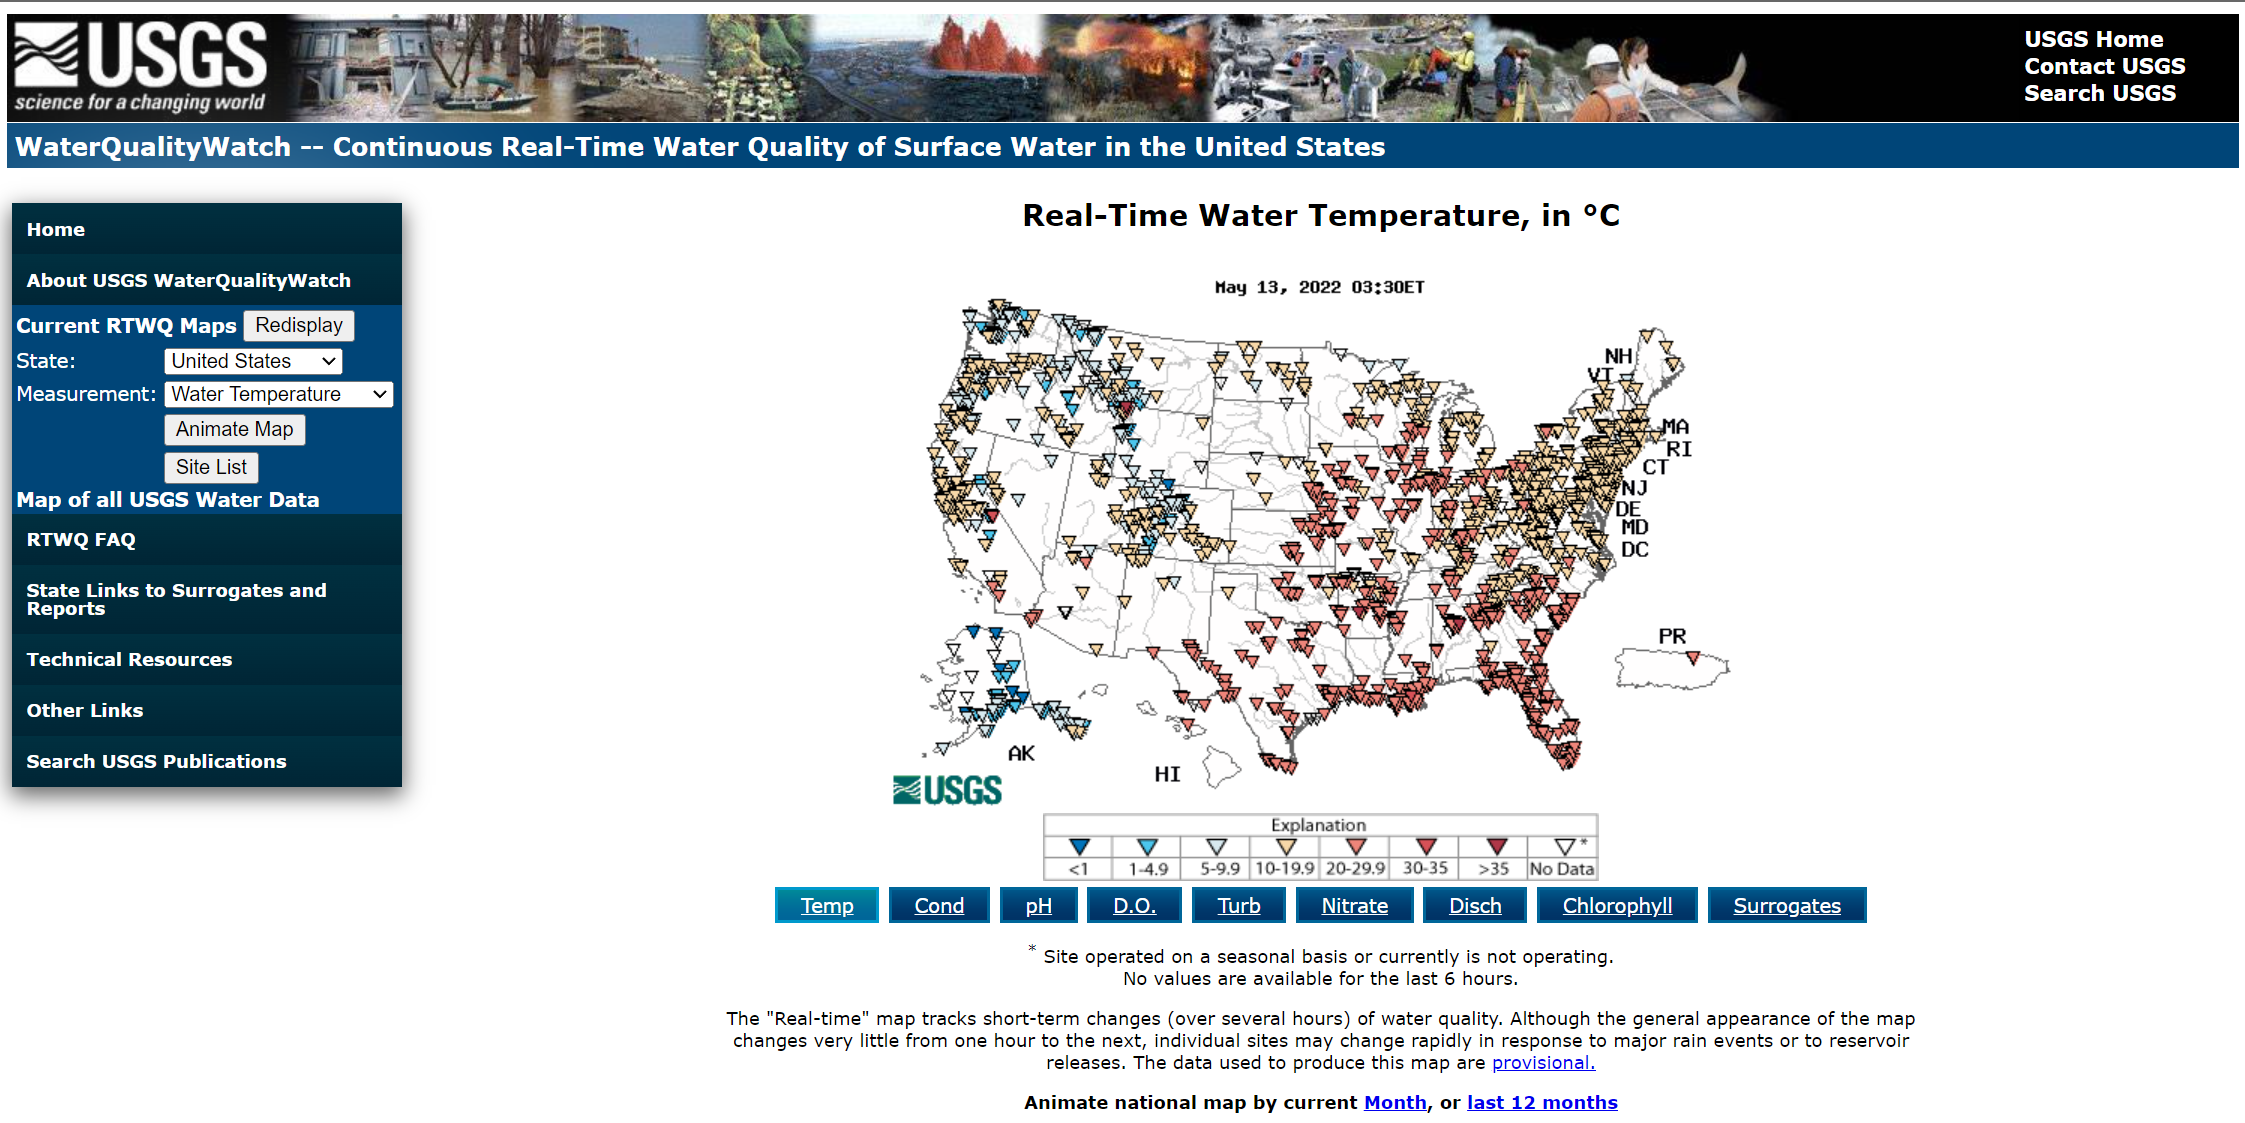
\includegraphics[scale=0.30]{figs/usgs_water.png}
        \caption{USGS WaterQualityWatch stations}
    \end{figure}

\paragraph{Data processing}
    The location chosen for analysis is \textit{ORIENT HARBOR AT ORIENT NY}, located at $41.13663889^\circ N$ and $-72.30675^\circ E$, accurate to $\pm .1 s$

    The rationale behind choosing this location was the easy availability of data for 2018-01-01 to 2021-12-31 and its closeness to the Atlantic ocean.

    Its closeness to the Atlantic ocean made it easy to obtain the subset of data from the ocean color dataset of Sea Surface Temperature(\textit{SST}) and Chlorophyll(\textit{Chlor\_a})

    \begin{figure}[H]
        \centering
        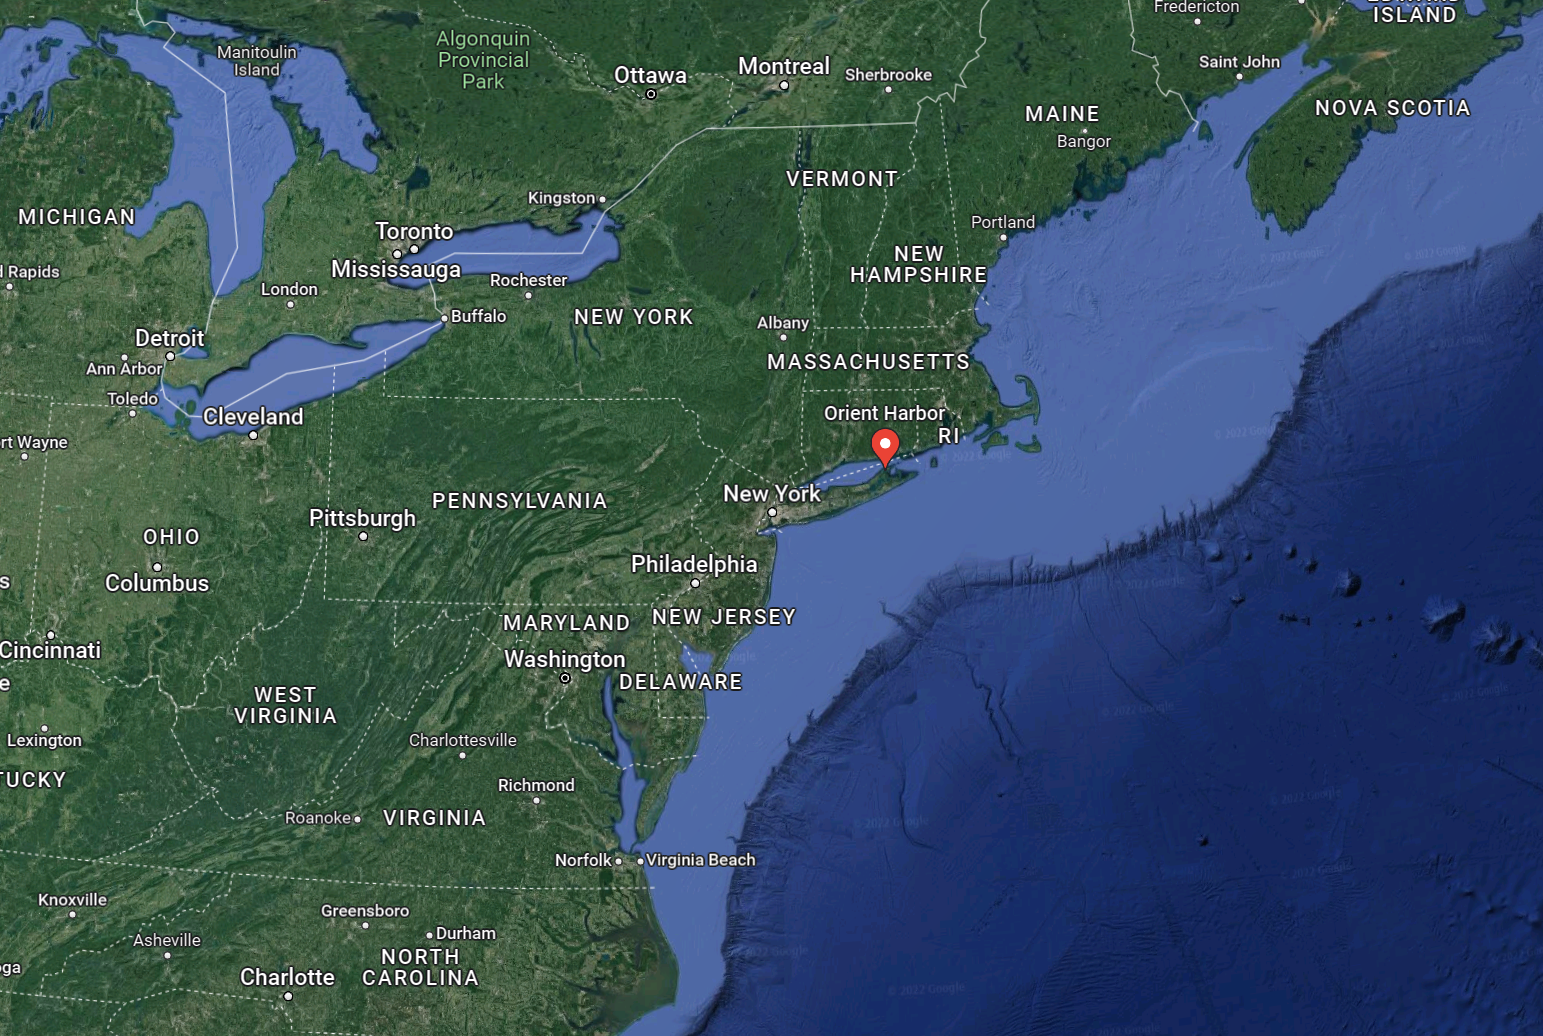
\includegraphics[width=10cm]{figs/RSS_SATELLITE_OBS.png}
        \caption{Satellite blown-up view}
    \end{figure}
    \begin{figure}[h]
        \centering        
        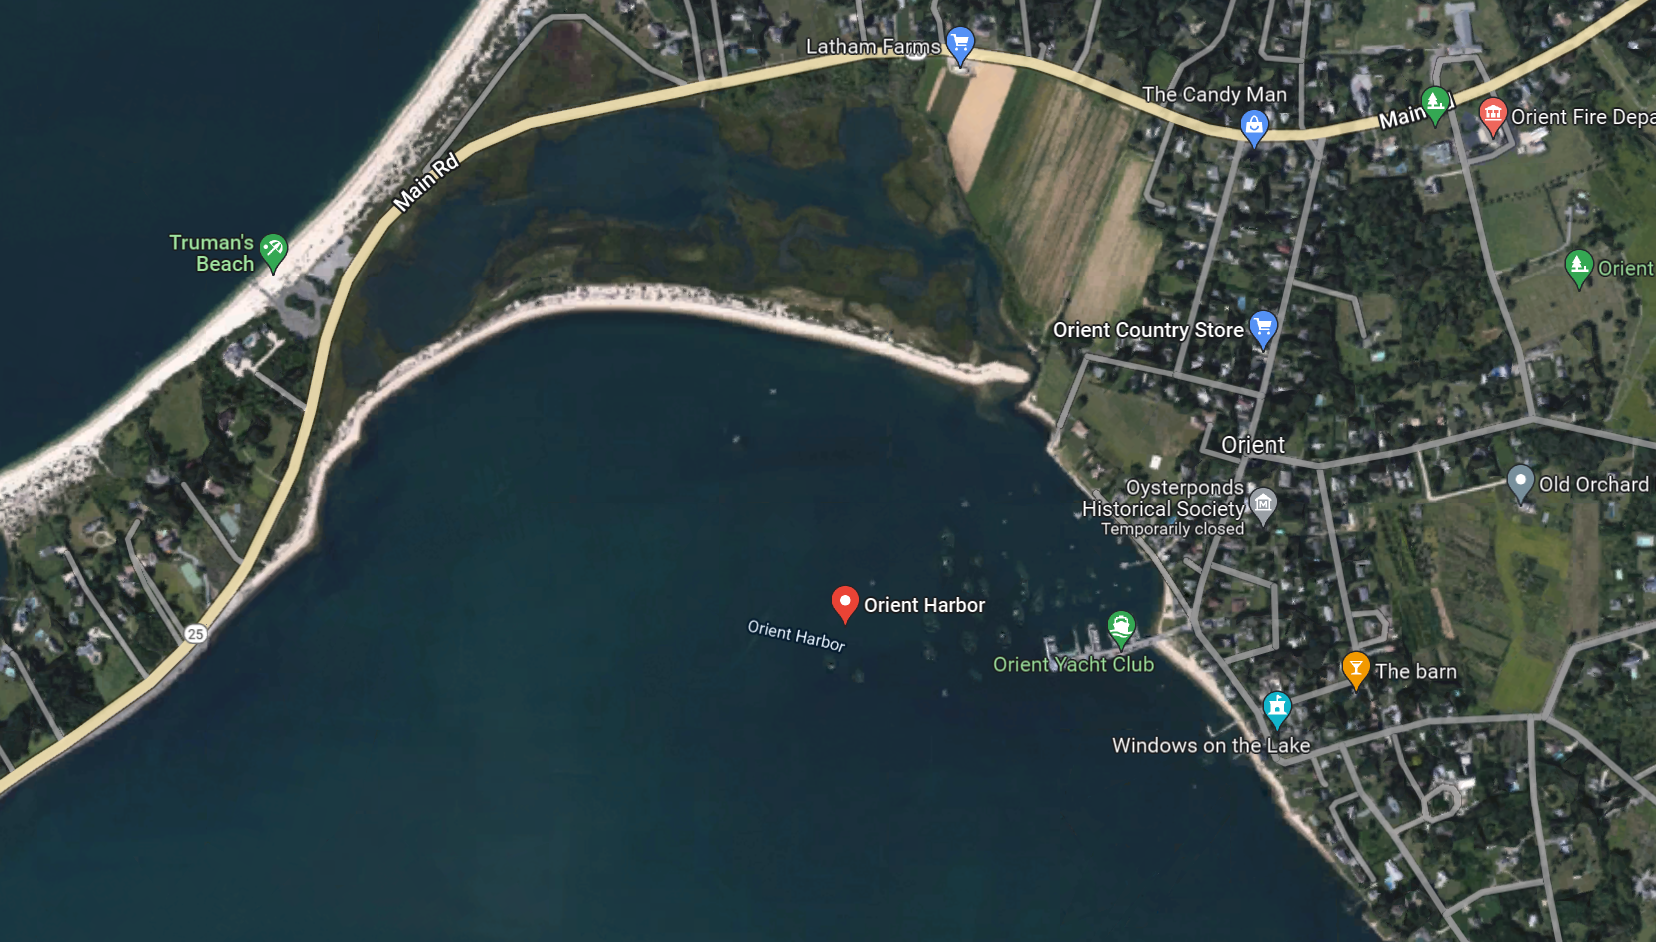
\includegraphics[width=10cm]{figs/RSS_OBS.png}
        \caption{Satellite close-up view}
    \end{figure}
    
    \paragraph{NOTE:}
    For better results and analysis choosing multiple locations with adequate separation would be ideal, but the turbidity and water contamination may bias our analysis, so we have restricted to a single location as a proof-of-concept.
